\chapter{动物吃什么}\label{ch:g2:what-animals-eat}

草地上的兔子整天啃草。黄昏时
穿过同一片草地的狐狸，对草根本不感兴趣，
它只对兔子感兴趣。乌鸫早上吃蠕虫，
下午吃樱桃。每种\omterm{def:g1:animals-around-us:animal}{动物}都必须进食，
但并非每种\omterm{def:g1:animals-around-us:animal}{动物}吃的东西都一样。

\section{三类动物的食性}

\begin{definition}[植食性动物、肉食性动物、杂食性动物]\label{def:g2:what-animals-eat:kinds}
\omterm{def:g1:animals-around-us:animal}{动物}可以按所吃的食物来分类：
\begin{itemize}
  \item \emph{植食性动物}\index{植食性动物}吃\omterm{def:g1:plants-around-us:plant}{植物}：草、
        叶、\omterm{def:g2:from-seed-to-plant:seed}{种子}、果实——兔子、牛、蜗牛；
  \item \emph{肉食性动物}\index{肉食性动物}吃其他\omterm{def:g1:animals-around-us:animal}{动物}：
        狐狸、猫、瓢虫（捕食
        微小的蚜虫）；
  \item \emph{杂食性动物}\index{杂食性动物}既吃\omterm{def:g1:plants-around-us:plant}{植物}，也吃
        \omterm{def:g1:animals-around-us:animal}{动物}：乌鸫、野猪——还有人类。
\end{itemize}
\end{definition}

\begin{example}[一片草地，三份食谱]\label{ex:g2:what-animals-eat:meadow}
在夏日的一片草地上：兔子啃草（\omterm{def:g2:what-animals-eat:kinds}{植食性动物}）；
狐狸捕食兔子（\omterm{def:g2:what-animals-eat:kinds}{肉食性动物}）；乌鸫此刻吃一条蠕虫，
稍后吃一颗樱桃（\omterm{def:g2:what-animals-eat:kinds}{杂食性动物}）。三位邻居，三份食谱——
注意，狐狸的这顿晚餐，它先吃过草。
\end{example}

\begin{omfigure}
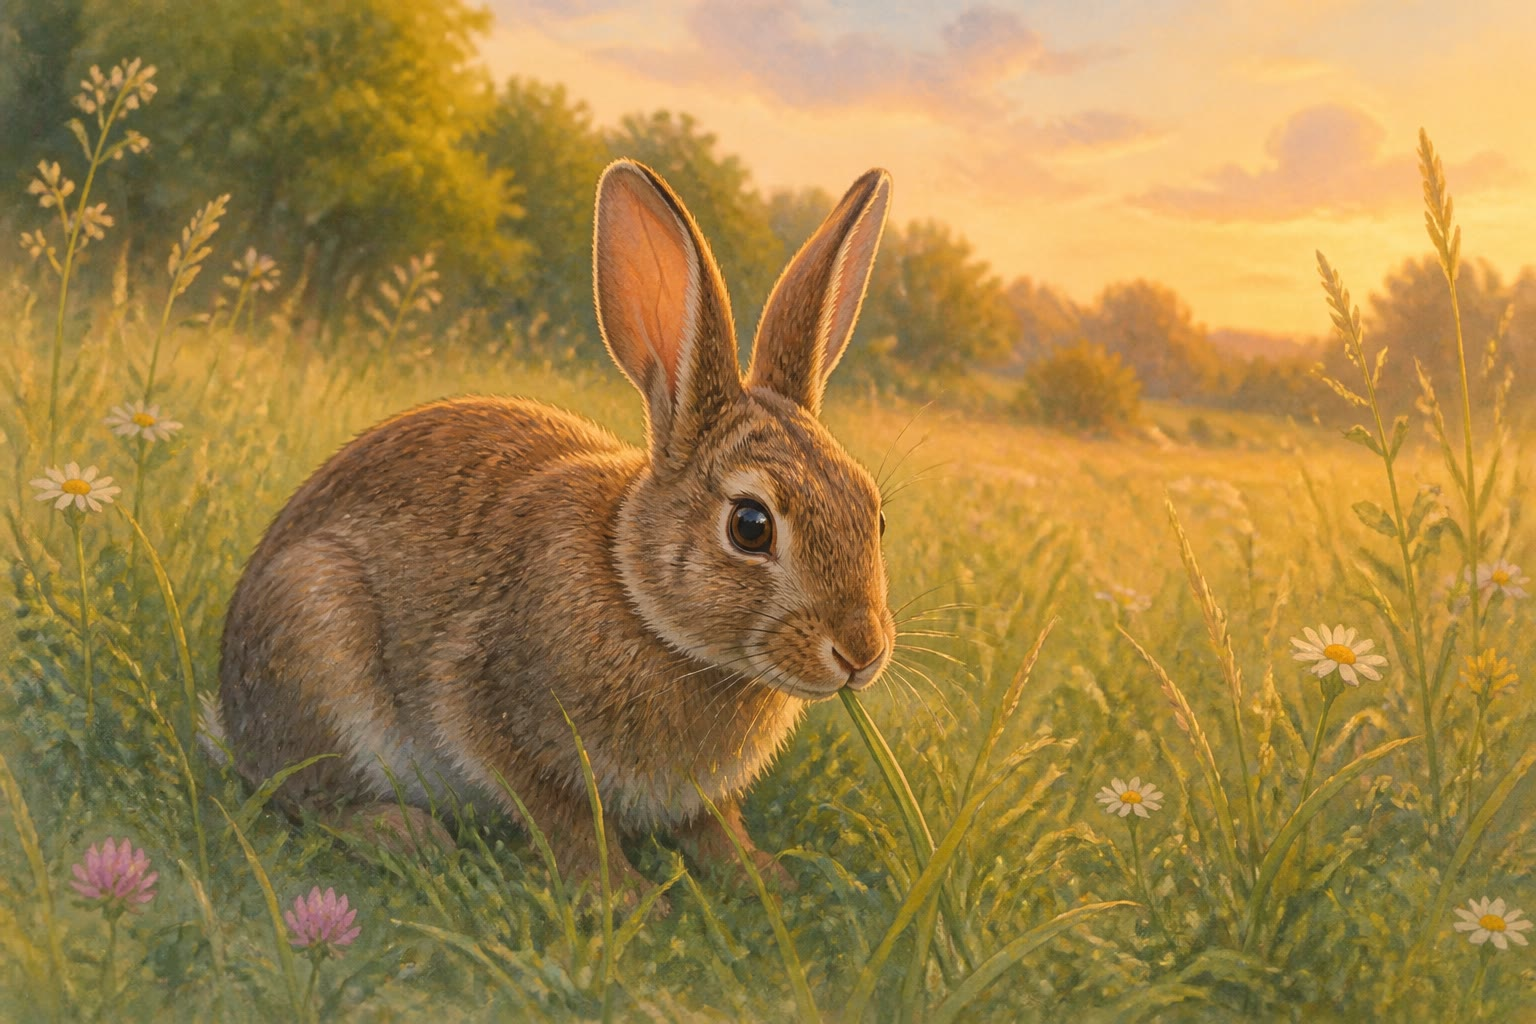
\includegraphics[width=0.6\linewidth]{images/book1/ai/g2-eat-rabbit.jpg}

{\small \omterm{def:g2:what-animals-eat:kinds}{植食性动物}在进食：兔子与草地，
一片叶接着一片叶。}
\end{omfigure}

\begin{remark}[肉食性动物并非坏人]\label{rem:g2:what-animals-eat:fox}
狐狸吃兔子并不“坏”，捕猎只是
\omterm{def:g2:what-animals-eat:kinds}{肉食性动物}的觅食方式——和兔子啃草一样自然。在
自然界中，吃与被吃是生命运作的一部分；后面的
一章会把这些进食串联成食物链。
\end{remark}

\section{从身体读出动物的食谱}

\begin{proposition}[身体与食谱相配]\label{prop:g2:what-animals-eat:match}
\omterm{def:g1:animals-around-us:animal}{动物}的身体藏着关于其食物的线索：
\begin{itemize}
  \item 像兔子和牛这样的\omterm{def:g2:what-animals-eat:kinds}{植食性动物}，有宽大扁平的
        臼齿用于磨碎\omterm{def:g1:plants-around-us:plant}{植物}，并且长时间
        进食；
  \item 像猫和狐狸这样的\omterm{def:g2:what-animals-eat:kinds}{肉食性动物}，有尖锐的牙齿用于
        抓住猎物，有锋利的爪子，以及用于
        捕猎的朝前的眼睛；
  \item 鸟类的喙能说明这一点：短而粗的喙用于
        啄碎\omterm{def:g2:from-seed-to-plant:seed}{种子}（麻雀），弯曲带钩的喙用于撕裂肉
        （鹰），细长的喙用于从树皮中挑出昆虫。
\end{itemize}
\end{proposition}
\admitted

\begin{omfigure}
\begin{minipage}[t]{0.31\linewidth}\centering
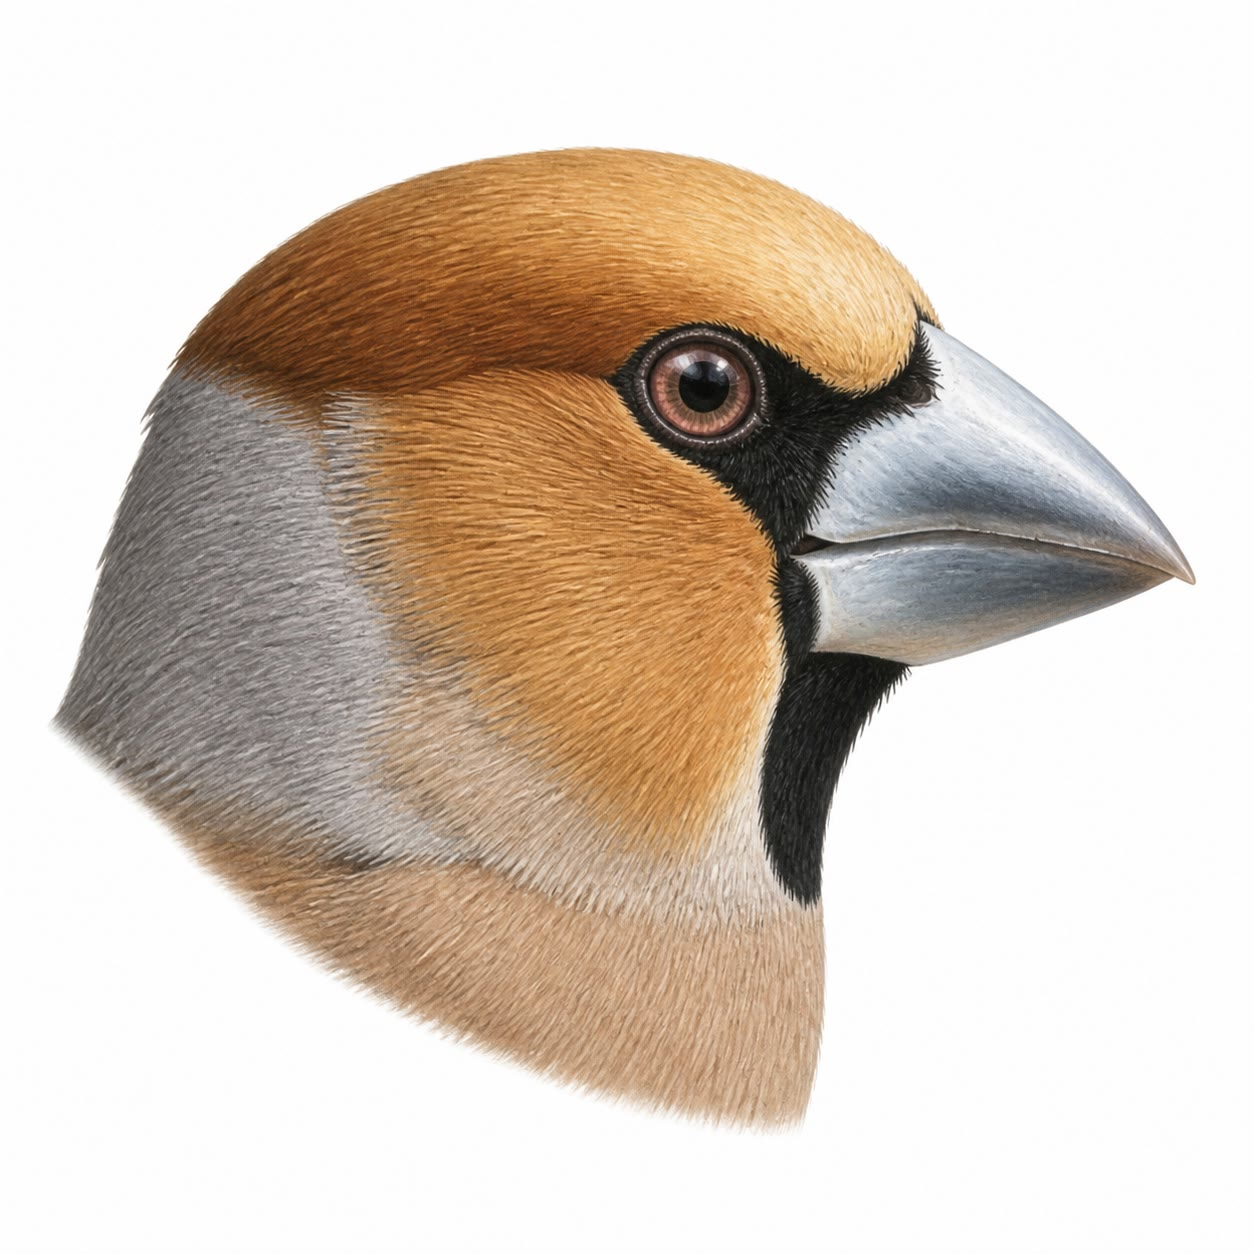
\includegraphics[width=\linewidth]{images/book1/ai/fig-beak-seed.jpg}

{\small 短粗的喙：\\ 啄碎\omterm{def:g2:from-seed-to-plant:seed}{种子}}
\end{minipage}\hfill
\begin{minipage}[t]{0.31\linewidth}\centering
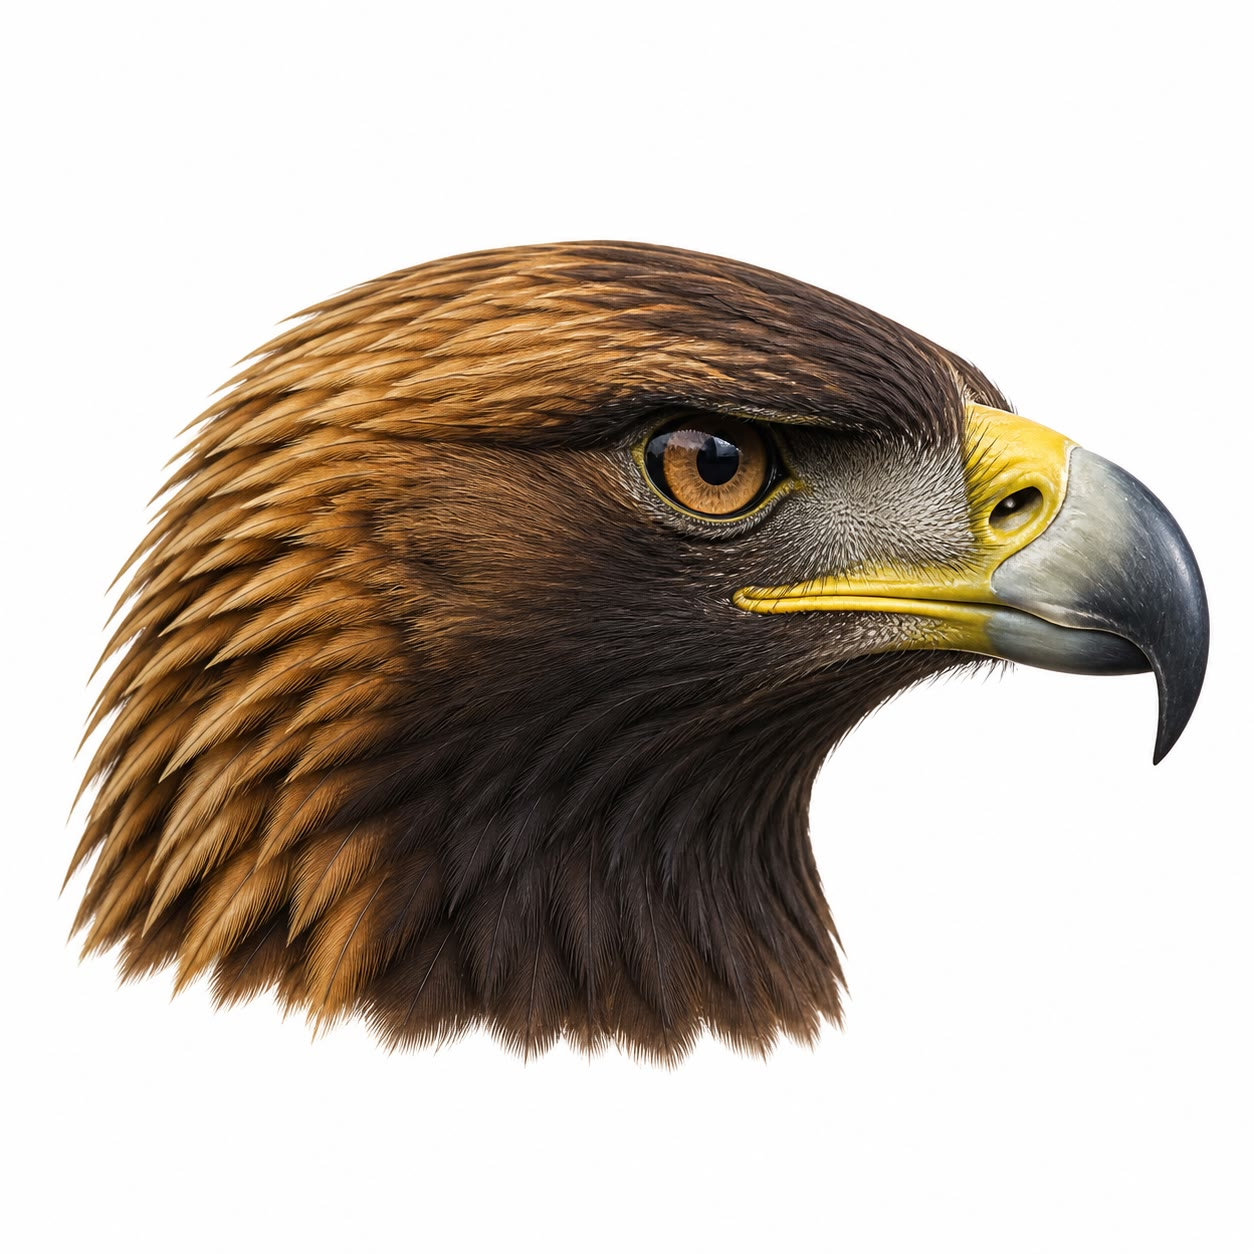
\includegraphics[width=\linewidth]{images/book1/ai/fig-beak-hook.jpg}

{\small 带钩的喙：\\ 撕裂肉}
\end{minipage}\hfill
\begin{minipage}[t]{0.31\linewidth}\centering
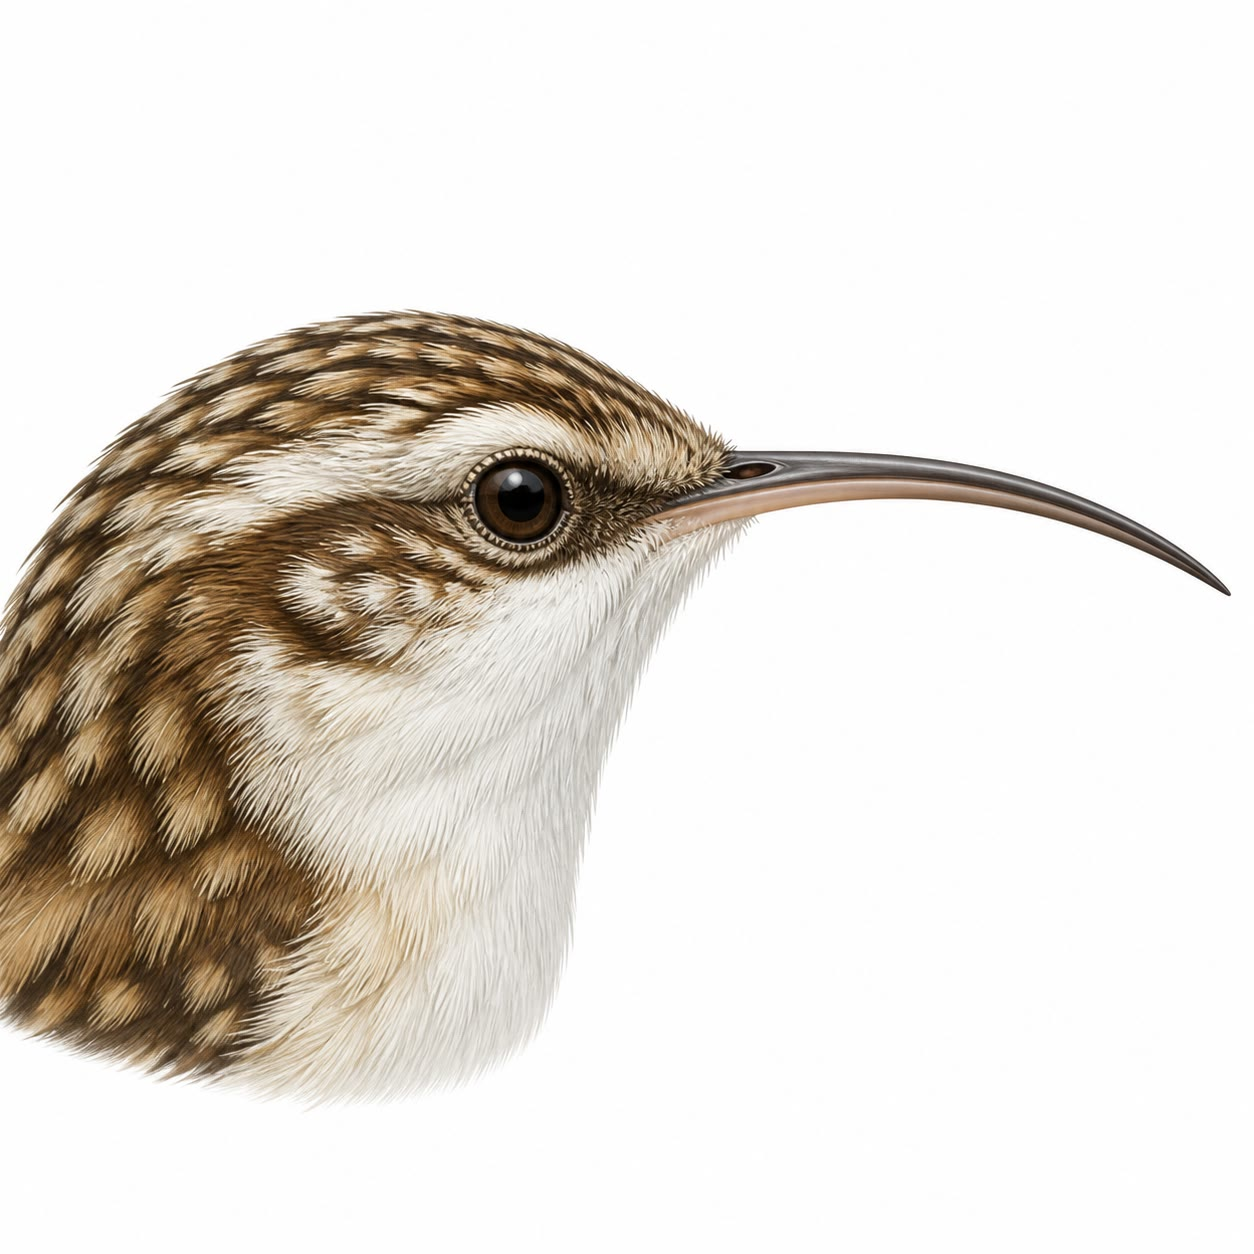
\includegraphics[width=\linewidth]{images/book1/ai/fig-beak-thin.jpg}

{\small 细长的喙：\\ 挑出昆虫}
\end{minipage}

\medskip
{\small 三种喙，三份食谱：鸟喙是由
食物塑造的工具。}
\end{omfigure}

\begin{example}[猫的牙齿]\label{ex:g2:what-animals-eat:cat}
看猫打哈欠：嘴的前角处有又长又尖的
牙齿。那是抓捕猎物的牙齿，\omterm{def:g2:what-animals-eat:kinds}{肉食性动物}的装备。
牛打哈欠时则看不到这些：它的口腔里
全是宽大扁平、用来磨草的臼齿。
\end{example}

\begin{method}[推测食谱]\label{met:g2:what-animals-eat:guess}
要推测一种未知\omterm{def:g1:animals-around-us:animal}{动物}吃什么：
\begin{enumerate}
  \item 看牙齿或喙：是扁平的磨齿、尖锐的抓齿，
        还是两者兼有？
  \item 看爪子和眼睛：它们是捕猎的工具吗？
  \item 如果可以，观察它进食——这是最可靠的线索；
  \item 最后判断它是植食性、肉食性还是\omterm{def:g2:what-animals-eat:kinds}{杂食性动物}。
\end{enumerate}
\end{method}

\section{日复一日地吃饱}

\begin{proposition}[进食是每日的任务]\label{prop:g2:what-animals-eat:daily}
食物是身体的燃料和建筑材料，因此\omterm{def:g1:animals-around-us:animal}{动物}必须
一次又一次地进食，日复一日。需要花多少时间
取决于食谱：草每一口提供的养分很少，所以牛
要吃好几个小时；肉的营养丰富，所以狐狸可能只吃一顿好饭就休息。
\end{proposition}
\admitted

\begin{example}[冬天的食谱变化]\label{ex:g2:what-animals-eat:winter}
食物随季节而变化。黑鸫在夏天吃蠕虫和
昆虫，但到了冬天，地面变硬时，它便改吃
浆果。\omterm{def:g2:what-animals-eat:kinds}{杂食性动物}食谱广泛，在日子变得艰难时
是极大的帮助。
\end{example}

\section{练习}

\begin{exercise}[$\star$]\label{exo:g2:what-animals-eat:1}
说出下列\omterm{def:g1:animals-around-us:animal}{动物}的名称：吃\omterm{def:g1:plants-around-us:plant}{植物}的\omterm{def:g1:animals-around-us:animal}{动物}；吃其他\omterm{def:g1:animals-around-us:animal}{动物}的\omterm{def:g1:animals-around-us:animal}{动物}；
两者都吃的\omterm{def:g1:animals-around-us:animal}{动物}。
\end{exercise}

\begin{exercise}[$\star$]\label{exo:g2:what-animals-eat:2}
判断下列\omterm{def:g1:animals-around-us:animal}{动物}分别属于植食性、肉食性还是\omterm{def:g2:what-animals-eat:kinds}{杂食性动物}：（a）牛；（b）狐狸；（c）
黑鸫；（d）蜗牛；（e）人？
\end{exercise}

\begin{exercise}[$\star$]\label{exo:g2:what-animals-eat:3}
\omterm{def:g2:what-animals-eat:kinds}{植食性动物}最需要哪一类牙齿：平坦的磨牙，
还是尖锐的抓牙？为什么？
\end{exercise}

\begin{exercise}[$\star$]\label{exo:g2:what-animals-eat:4}
将每种喙与一种食谱配对：短而粗；弯而钩；
长而细。
\end{exercise}

\begin{exercise}[$\star$]\label{exo:g2:what-animals-eat:5}
瓢虫体型小，外形漂亮，却是\omterm{def:g2:what-animals-eat:kinds}{肉食性动物}。
它捕食什么？
\end{exercise}

\begin{exercise}[$\star$]\label{exo:g2:what-animals-eat:6}
为什么牛吃东西的时间比狐狸长得多？
请利用\cref{prop:g2:what-animals-eat:daily}。
\end{exercise}

\begin{exercise}[$\star$]\label{exo:g2:what-animals-eat:7}
黑鸫在夏天和冬天分别吃什么？
为什么食谱广泛是有用的？
\end{exercise}

\begin{exercise}[$\star$]\label{exo:g2:what-animals-eat:8}
试一试：在公园或喂食器旁观察鸟类，记录每种鸟吃的东西，
即\omterm{def:g2:from-seed-to-plant:seed}{种子}、面包、昆虫、浆果，并观察它们的喙。
\cref{prop:g2:what-animals-eat:match}是否成立？
\end{exercise}

\begin{exercise}[$\star\star$]\label{exo:g2:what-animals-eat:9}
\omterm{def:g1:animals-around-us:animal}{动物}园收到一只来历不明的\omterm{def:g1:animals-around-us:animal}{动物}：前牙尖锐，
爪子锋利，眼睛朝前。它最可能的食谱是什么？
你用了\cref{met:g2:what-animals-eat:guess}中的哪些步骤？
\end{exercise}

\begin{exercise}[$\star\star$]\label{exo:g2:what-animals-eat:10}
“没有草，很快就不会有狐狸了。”
狐狸从不吃草，但这句话是对的。请结合
\cref{ex:g2:what-animals-eat:meadow}中的草地加以解释。
\end{exercise}
